
\natp{Add basics about copulas, Sklar's Theorem}

Currently: Archimedean (Clayton, Gumbel), Gaussian, NVM / elliptical
(Student $t$, NIG), NIG factor

Possibly: double $t$, Frank, skewed-$t$



\subsection{Gaussian Copula}\label{subsec:Gaussian-copula}

The {\bf Gaussian copula}, also called {\bf Normal
    copula}, is the copula generated by jointly normally
  distributed random variables (given here in bivariate form):
\begin{equation*}
  C_{\rho,\Ncdf}(u,v) := \Ncdf_2(\Ncdf^{(-1)}(u), \Ncdf^{(-1)}(v);
  \rho), 
\end{equation*}
where $\Ncdf_2$ and $\Ncdf$ are the bivariate and univariate normal
distribution functions, respectively, and $\rho $ is the correlation
parameter. 
\begin{figure}[t]
  \centering
  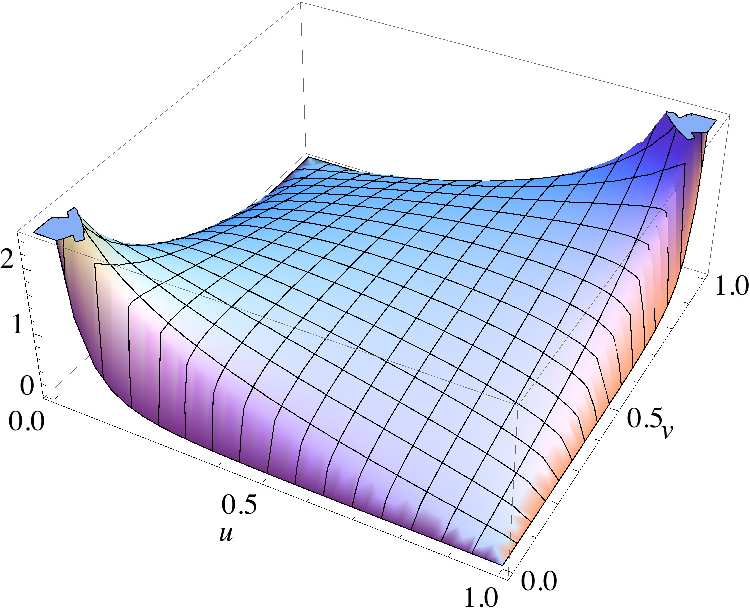
\includegraphics[scale=.35]{_pics/copulas/normal1.pdf}  
  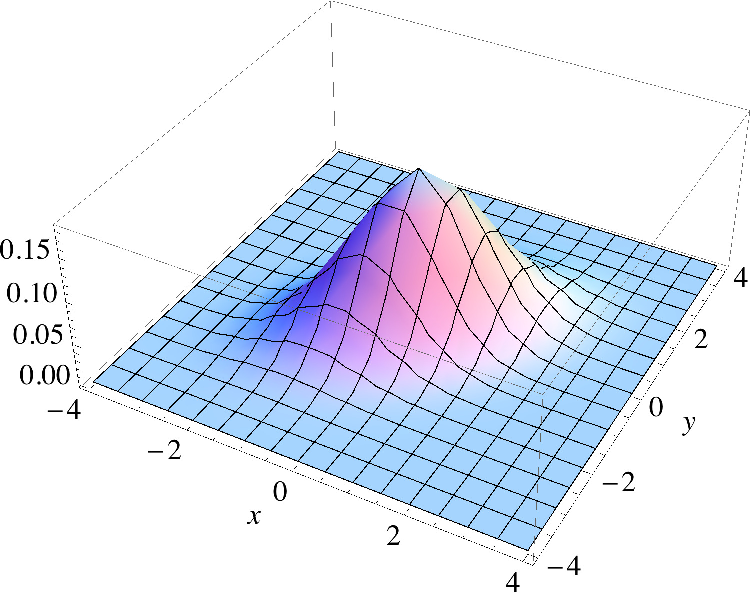
\includegraphics[scale=.35]{_pics/copulas/normal2.pdf}  
  \caption{Left: Density of the Gaussian (Normal) copula. Right:
    Density of the bivariate Normal distribution ($\rho=0.5$ in both
    cases).} 
  \label{fig:normalcopula}
\end{figure}

The Gaussian or Normal copula is
\begin{align}
    C^{Ga}_\Sigma(x) &= \frac{1}{(2\pi)^{d/2} |\Sigma|^{1/2}}
    \int_{-\infty}^{\Phi^{-1}(x_1)} \dots \int_{-\infty}^{\Phi^{-1}(x_d)}
    \exp \left\{
    -\frac{1}{2}y^\top \Sigma^{-1}y
    \right\}
    dy_1 \dots dy_d, \quad x\in \R^d.
    \end{align}

The copula density is
\begin{align}
    c^{Ga}_\Sigma(x) &= \frac{1}{(2\pi)^{d/2} |\Sigma|^{1/2}}
    \exp \left\{
    -\frac{1}{2}\begin{pmatrix} \Phi^{-1}(x_1) \\ \vdots \\ \Phi^{-1}(x_d) \end{pmatrix}^\top \Sigma^{-1} \begin{pmatrix} \Phi^{-1}(x_1) \\ \vdots \\ \Phi^{-1}(x_d) \end{pmatrix}
    \right\}
    \end{align}

Simplified notation bivariate Gaussian copula
\begin{align}
       C^{Ga}_\rho \{w, g(w)\} &= \Phi_\rho [\Phi^{-1}(w), \Phi^{-1}\{g(w)\}],
\end{align}
where $g(w): [0,1] \mapsto \mathbb{R}$ is defined above,
$\rho$ is the dependency parameter of a bivariate Gaussian copula,
$\Phi_\rho$ is bivariate normal distribution with mean 0 and covariance $\begin{bmatrix}1 & \rho \\ \rho & 1 \end{bmatrix}$,
$\Phi(\cdot)$ is CDF of standard normal,
$\phi(\cdot)$ is PDF of standard normal,
$\Phi^{-1}(\cdot)$ is quantile function of standard normal.

\natp{\em [I suggest to move the part below to the section where the
  formula for $R^h$ is discussed. Also, there is a simpler version
  that requires only univariate function evluations.]}

The bivariate $D_1 C^{Ga}\{w, g(w)\}$ is
\begin{align}
    D_1 C^{Ga}_\rho\{w, g(w)\} = \int_{-\infty}^{\Phi^{-1}\{g(w)\}} \phi_\rho\{
    \Phi^{-1}(w), u \}du \cdot \frac{1}{\phi\{\Phi^{-1}(w)\}}
    \end{align}
\begin{proof}
    \begin{align}
    D_1 C_\rho\{w, g(w)\}
    &= \left. \frac{\partial C_\rho\{w, g(w')\}}{\partial w}\right|_{w'=w}\\
    &= \left. \frac{\partial \Phi_\rho [\Phi^{-1}(w), \Phi^{-1}\{g(w)\}]}{\partial \Phi^{-1}(w)} \frac{\partial \Phi^{-1}(w)}{\partial w}\right|_{w'=w}\\
    &= \frac{1}{2\pi\rho} \int_{-\infty}^{\Phi^{-1}\{g(w)\}} \exp\left\{
        -\frac{1}{2(1-\rho^2)} \Phi^{-1}(w)^2 - 2\rho\Phi^{-1}(w)u + u^2
        \right\}du
        \cdot \frac{1}{\phi\{\Phi^{-1}(w)\}}
        \end{align}
    \end{proof}

% The bivariate Gaussian Copula density~$c^{Ga}\{w, g(w)\}$ is
% \begin{align}
%     c_\rho^{Ga}\{w, g(w)\} &= \frac{\partial D_1C_\rho^{Ga}\{w, g(w)\}}{\partial g(w)}\\
%                            &= \frac{\phi_\rho [\Phi^{-1}(w), \Phi^{-1}\{g(w)\}]}
%                             {\phi\{\Phi^{-1}(w)\}\phi[\Phi^{-1}\{g(w)\}]}
%     \end{align}


    
\subsubsection*{Hedge distribution}
\label{sec:hedge-distribution-gaussian}

Let $R^S\sim \Ncdf(\mu_S, \sigma_S^2)$ and $R^F\sim \Ncdf(\mu_F,
\sigma_F^2)$ and assume further that they are jointly normally
distributed with correlation $\rho$. Then,
\begin{equation*}
  R^h = R^S - h R^F \sim \Ncdf(\mu_S - h \mu_F, \sigma_s^2 + h^2
  \sigma_F^2 - 2\rho h \sigma_S \sigma_F).
\end{equation*}
More generally, if $R^k\sim F^k$, $k\in \{S,F\}$, then the
distribution of $R^h$ can be expressed with univariate
expressions: 
\begin{align*}
  \p(R^S-h R^F\leq x)
  &= 1-\E\left[ \p\left(R^F\leq \frac{R^S-x}{h}\big| R^S\right)\right] \\ %
  &= 1-\E\left[\p \left(\Ncdf^{(-1)}(F_F(R^F)) \leq
    \Ncdf^{(-1)}\left(F_F\left(\frac{R^S-x}{h}\right)\right) \Big|
    R^S\right)\right] \\%
  &= 1-\E\left[ \p\left(\rho \Ncdf^{(-1)}(F_S(R^S)) + \sqrt{1-\rho^2}
    \varepsilon \leq \Ncdf^{(-1)}\left(F_F\left(\frac{R^S-x}{h}\right)\right) \Big|
    R^S\right)\right]\\ %
  &= 1-\E\left[ \Ncdf \left(
    \frac{\Ncdf^{(-1)}\left(F_F\left(\frac{R^S-x}{h}\right)\right) -\rho
    \Ncdf^{(-1)}(F_S(R^S))} { \sqrt{1-\rho^2}}\right)\right]\\
  &= 1-\int_0^1  \Ncdf \left(
    \frac{\Ncdf^{(-1)}\left(F_F\left(\frac{F_S^{(-1)}(u)-x}{h}\right)\right) -\rho
    \Ncdf^{(-1)}(u)} { \sqrt{1-\rho^2}}\right) \,\dd u.
\end{align*}



\subsection{Archimedean copulas}
\label{sec:archimedean-copulas}

\begin{itemize}
\item A well-studied one-parameter family of copulas are the {\bf 
    Archimedean copulas}. 
\item Let $\phi:[0,1]\rightarrow[0,\infty]$ be a
  continuous and strictly decreasing function with $\phi(1)=0$ and
  $\phi(0)\leq\infty$.
\item  We define the {\bf pseudo-inverse} of $\phi$ as 
  \begin{equation*}
    \phi^{(-1)}(t)=
    \begin{cases}
      \phi^{-1}(t), &0\leq t\leq \phi(0),\\
      0, &\phi(0)<t\leq\infty.
    \end{cases}
  \end{equation*}
\item If, in addition, $\phi$ is convex, then the following function
  is a copula: 
  \begin{equation*}
    C(u,v)=\phi^{(-1)}(\phi(u)+\phi(v)).
  \end{equation*}
  \vspace*{-\baselineskip}
\item Such copulas are called {\bf Archimedean copulas}, and the
  function $\phi$ is called an {\bf Archimedean copula generator}. 
\item Examples of Archimedean copulas are the {\bf Gumbel} and the
  {\bf Clayton} copulas:
  \begin{align*}
    C_{\theta,{\rm Gu}}(u,v) &= \exp\left\{-((-\ln u)^\theta + (-\ln
                               v)^\theta)^{1/\theta}\right\},& 1\leq \theta<\infty,\\
    C_{\theta,{\rm Cl}}(u,v)&= (u^{-\theta} + v^{-\theta}
                              -1)^{-1/\theta}, & 0<\theta<\infty. 
  \end{align*}
\item In the case of the Gumbel copula, the independence copula is 
  attained when $\theta=1$ and the comonotonicity copula is attained
  as $\theta\rightarrow\infty$. 
\item Thus, the Gumbel copula interpolates between independence and
  perfect dependence.  
\item In the case of the Clayton copula, the independence copula is
  attained as $\theta\rightarrow 0$, whereas the comonotonicity
  copula is attained as $\theta\rightarrow\infty$. 
\end{itemize}

\subsection{Elliptical Copulas and normal variance mixtures}
\label{subsec:elliptical-copulae}


\providecommand{\bZ}{\ensuremath{\bm{Z}}}
\providecommand{\bU}{\ensuremath{\bm{U}}}
\providecommand{\bu}{\ensuremath{\bm{u}}}

See e.g.\ Theorem 3.22, Definition 3.26 and Theorem 3.28 of
\citep{McNeil2005}:
\begin{definition}
  A random vector $\bZ=(Z_0,\ldots, Z_d)^T$ follows an elliptical
  distribution if it has a representation
  \begin{equation*}
    \bZ\stackrel{\mathcal L}= G A \bU,
  \end{equation*}
  where $G>0$ is a scalar random variable, the so-called {\em mixing
  variable}, $A$ is a deterministic $(d+1)\times (d+1)$ matrix with
$A A^T:=\Sigma$, which in turn is a $(d+1)\times (d+1)$ nonnegative
definite symmetric matrix of rank $d+1$, and $\bU$ is a
$(d+1)$-dimensional random vector uniformly distributed on the unit
sphere $\mathcal S_{d+1}:=\{\bm{z}\in \R^{d+1}: \bm z^T \bm z=1\}$,
and $\bU$ is independent of $G$.
\end{definition}

A subclass of elliptical distributions are the so-called {\em normal
  variance mixtures (NVM)}, see Section 3.3 of \citep{McNeil2005}. For the
connection between NVM and elliptical distributions, see also Theorem
3.25 of \citep{McNeil2005}. 

\begin{definition}[Normal variance mixture (NVM)]
  The random vector $\mathbf X=(X_1, \ldots, X_k)^T$ follows a
  multivariate {\em normal variance mixture (NVM) distribution} if
  \begin{equation*}
    \mathbf X \stackrel{\mathcal L}{=} \mathbf \mu + \sqrt{W} A\mathbf
    Z, 
  \end{equation*}
  where
  \begin{enumerate}[(i)]
  \item $\mathbf Z\sim \Ncdf_k(\mathbf 0, I_k)$, i.e., $\mathbf Z$ are
    independent, standard normally distributed,
  \item $W\geq 0$ is a random variable independent of $\mathbf Z$,
  \item $A\in \R^{d\times k}$ and $\mathbf \mu\in R^d$ are a matrix
    and vector of constants, respectively. 
  \end{enumerate}
\end{definition}

It is easily observed that $\mathbf X|W=w \sim \Ncdf_d(\mathbf \mu,
w\Sigma)$, where $\sigma = A A'$.

In general, we will assume that $\Sigma$ is positive definite and that
$W>0$ $\pas$. Then, the density of $\mathbf X$ is given by
\begin{align*}
  f(\mathbf x) &= \int f_{\mathbf X|W} (\mathbf x|w)\, \dd H(w)\\
  &= \int \frac{w^{-d/2}} {(2\pi)^{d/2} |\Sigma|^{1/2}} \exp\left( -
    \frac{(\mathbf x-\mathbf \mu)' \Sigma^{-1} (\mathbf x-\mathbf
    \mu)} {2w} \right)\, \dd H(w),
\end{align*}
where $H$ is the distribution function of $W$.

Special cases:
\begin{itemize}
\item Normal distribution: $W$ constant
\item Student $t$ distribution: $W\sim \displaystyle Ig(1/2 \nu, 1/2
  \nu)$, where $Ig$ is an inverse gamma distribution
\item Symmetric generalised hyperbolic distribution: $W\sim
  N^{-}(\lambda, \chi, \psi)$ where $N^{-}$ refers to
  the generalised inverse Gaussian (GIG) distribution;
\item Normal inverse Gaussian (NIG): $W$ follows a GIG distribution
  with $\lambda=-0.5$.  
\end{itemize}

Copulas are obtained from elliptical distributions via Sklar's theorem
by transforming the margins to uniforms. 

\subsubsection*{Hedge distribution}
\label{sec:hedge-distribution-1}

Let $(R^S, R^F)$ follow a normal variance mixture, i.e., there exists a
decomposition such that
\begin{align*}
  R^S &=\mu_S + \sqrt{W} \sigma_S Z_1\\
  R^F &= \mu_F + \sqrt{W} \sigma_F (\rho Z_1 + \sqrt{1-\rho^2} Z_2),
\end{align*}
where $W$ is the mixing variable and $Z_1, Z_2$ are independent
standard normal variables. Then, $R^h$ follows a NVM distribution with
\begin{equation*}
  R^h = R^S - h R^F =  \mu_S - h \mu_F + \sqrt{W}
  \left((\sigma_S-h\sigma_F\rho)Z_1 -h \sqrt{1-\rho^2} 
    \sigma_F Z_2\right) = \mu_S - h \mu_F + \sqrt{W} Z_3,
\end{equation*}
where $Z_3\sim \Ncdf(0, \sigma_S^2 + h^2\sigma_F^2 - 2\rho
h\sigma_S \sigma_F)$. 

More generally, let $R^k\sim F^k$, $k\in \{S,F\}$ and write $V$
as the marginal distribution functions of the NVM distribution
components. Let $V^{(-1)}(F_S(R^S)) \stackrel{\mathcal L}{=} \sqrt{W}
Z_1$ and $V^{(-1)}(F_F(R^F)) \stackrel{\mathcal L}{=} 
\sqrt{W} \rho Z_1 + \sqrt{W} \sqrt{1-\rho^2} Z_2$, were $Z_1, Z_2$ are
independent standard normals. Then 
\begin{align*}
  \p(R^S-h R^F\leq x)
  &= 1-\E\left[ \p\left(R^F\leq \frac{R^S-x}{h}\big| R^S\right)\right] \\ %
  &= 1-\E\left[\p \left(V^{(-1)}(F_F(R^F)) \leq
    V^{(-1)}\left(F_F\left(\frac{R^S-x}{h}\right)\right) \Big|
    W, Z_1\right)\right] \\%
  &= 1-\E\left[ \p\left(\sqrt{W} \rho Z_1 + \sqrt{W} \sqrt{1-\rho^2}
    Z_2\leq V^{(-1)}\left(F_F\left(\frac{F_S^{(-1)}(V(\sqrt{W}
    Z_1))-x}{h}\right)\right) \Big| W, Z_1\right)\right]\\ %
  &= 1-\E\left[ \Ncdf \left(
    \frac{V^{(-1)}\left(F_F\left(\frac{F_S^{(-1)}(V(\sqrt{W}
    Z_1))-x}{h}\right)\right) -\rho \sqrt{W} Z_1} {
    \sqrt{W}\sqrt{1-\rho^2}}\right)\right]\\ 
  &= 1-\int_0^\infty \int_{-\infty}^{\infty} \Ncdf \left(
    \frac{V^{(-1)}\left(F_F\left(\frac{F_S^{(-1)}(V(\sqrt{w}
    z_1))-x}{h}\right)\right) -\rho\sqrt{w} z_1} { \sqrt{w}
    \sqrt{1-\rho^2}}\right) \, \varphi(z_1)\, f_W(w)\, \dd z_1\, \dd
    w.% \\
  % &= 1-\int_0^1 \int_{-\infty}^\infty  \Ncdf \left(
  %   \frac{V^{(-1)}\left(F_F\left(\frac{F_S^{(-1)}(u)-x}{h}\right)\right)
  %   -\rho V^{(-1)}(u)} { V^{(-1)}(u)/z_1
  %   \sqrt{1-\rho^2}}\right) \, \varphi(z_1)\, \dd z_1\, \dd
  %   u\\
\end{align*}
As in the Gaussian copula case, this expression contains evaluations
of only univariate distribution function. 


\subsection{Normal inverse Gaussian factor copula model}
\label{sec:norm-inverse-gauss-1}

\subsubsection{Normal inverse Gaussian distribution}
\label{sec:norm-inverse-gauss-2}


It was established in the previous section that a multivariate normal
inverse Gaussian (NIG)
distribution is a normal variance mixture. Here the random components 
have a joint scalar mixing variable. 
An additional copula model can be derived as a factor model from the
NIG distribution: under certain conditions, its distribution type is
preserved under linear combinations. This property, together with 
its infinite divisibility, allow for the construction of L\'evy
processes from NIG distributions. 

Following \citep{BarndorffNielsen1997}, a normal inverse Gaussian
(NIG) distribution has density function
\begin{equation*}
  g(x; \alpha,\beta, \mu, \delta) = \frac{\alpha}{\pi} \e^{\delta
    \sqrt{\alpha^2-\beta^2} -\beta\mu} \frac{1}{q((x-\mu)/\delta)}
  K_1\left[\delta \alpha q\left(\frac{x-\mu}{\delta}\right) \right]
  \e^{\beta x},\quad x>0,
\end{equation*}
where $q(x) = \sqrt{1+x^2}$ and where $K_1$ is the modified Bessel
function of third order and index $1$. The parameters satisfy $0\leq
|\beta|\leq \alpha$, $\mu\in \R$ and $\delta>0$. The parameters have
the following interpretation: $\mu$ and $\delta$ are location and
scale parameters, respectively, $\alpha$ determines the heaviness of
the tails and $\beta$ determines the degree of asymmetry. If
$\beta=0$, then the distribution is symmetric around $\mu$. 

The moment-generating function of the NIG distribution is given by
\begin{equation*}
  M(u; \alpha, \beta, \mu, \delta) = \exp\left( \delta
    \left(\sqrt{\alpha^2-\beta^2} - \sqrt{\alpha^2 - (\beta +
        u)^2}\right) + \mu u\right). 
\end{equation*}
As a direct consequence, moments are easily calculated with the
expectation and variance of the NIG distribution being
\begin{align}
  \label{eq:4}
  \mathbb E X &= \mu + 
                \frac{\delta \beta}{\sqrt{\alpha^2-\beta^2}}\\
  \label{eq:5}
  \text{Var}(X) &= \frac{\alpha^2\delta}{(\alpha^2-\beta^2)^{3/2}}.
\end{align}


Let $\text{IG}(\delta,\gamma)$ denote the {\em inverse Gamma
  distribution} with density function\footnote{%
  The density of the IG distribution in {\tt Mathematica} is given as
  \begin{equation*}
    f(x) = \sqrt{\frac{\lambda}{x^3}} \frac{1}{\sqrt{2\pi}}
    \e^{-\frac{\lambda(x-\mu)^2}{2 x\mu^2}},\quad x>0,
  \end{equation*}
  with parameters $\mu=\delta/\gamma$ and $\lambda=\delta^2$. 
  }%
\begin{equation}
  \label{eq:2}
  d(w; \delta, \gamma) = \frac{1}{\sqrt{2\pi}} \exp(\delta \gamma)
  w^{-3/2} \exp(-\frac{\delta^2/w + \gamma^2 z}{2}). 
\end{equation}
The $\text{NIG}(\alpha, \beta, \mu\, \delta)$ distribution is a normal
variance-mean mixture: $X$ follows an
$\text{NIG}(\alpha,\beta,\mu,\delta)$ distribution if $X$ conditional
on $W$ follows a normal distribution with mean $\mu+\beta W$ and
variance $W$, i.e., 
\begin{equation*}
  X|W\stackrel{\mathcal L}\sim \Ncdf(\mu + \beta W, W),
\end{equation*}
where $W$ follows an $\text{IG}(\delta, \sqrt{\alpha^2-\beta^2})$
distribution. 

It is easily seen from the moment-generating function that linear
combinations of NIG random variables are again NIG-distributed
provided they share the parameters $\alpha$ and $\beta$. Let $X_i\sim
\text{NIG}(\alpha, \beta, \mu_i, \delta_i)$, $i=1,2$, be
independent NIG variables. Then, 
\begin{equation*}
  \E\left[\e^{u(X_1+X_2)}\right] = \E\left[\e^{u X_1}\right]
  \E\left[\e^{u X_2}\right] = \exp\left((\delta_1+\delta_2)
    \left(\sqrt{\alpha^2-\beta^2} - \sqrt{\alpha^2 -
        (\beta+u)^2}\right) + (\mu_1+\mu_2) u\right),
\end{equation*}
hence $X_1+X_2\sim \text{NIG}(\alpha, \beta, \mu_1+\mu_2,
\delta_1+\delta_2)$. (This is also a direct consequence from the
properties of 
the normal inverse Gaussian L\'evy process $X_t$, which may be
represented as Brownian motion with a random time change,
\begin{equation*}
  X_t = B_{W_t} + \mu t,
\end{equation*}
where $B=(B_t)_{t\geq 0}$ is a Brownian motion and $W=(W_t)_{t\geq 0}$
is a L\'evy process with density given by \eqref{eq:2}. The random
variable $W_t$ can be interpreted as a first-passage time of an
independent Brownian motion $\overline B$, i.e., $W_t=\inf\{s>0:
\overline B_s + \sqrt{\alpha^2-\beta^2}s = \delta t\}$.)

As a consequence, the NIG distribution gives rise to two copulas:
\begin{itemize}
\item a copula determined from a linear combination of independent NIG
  random variables with identical parameters $\alpha, \beta$
  (essentially a factor model);
\item a copula determined from the multivariate normal-mean-variance
  mixture, which is a linear combination of normal random variables
  scaled by one scalar inverse Gaussian random variable.
\end{itemize}

\subsubsection{NIG factor copula}
\label{sec:nig-factor-copula}

We consider a simple factor model consisting of NIG-distributed random
variables.
\begin{proposition}
  \label{prop:NIG}
  Let $Z\sim \text{NIG}(\alpha, \beta, \mu, \delta)$ and
  $Z_i\sim \text{NIG}(\alpha, \beta, \mu_i, \delta_i)$,
  $i=1,\ldots, n$ be independent NIG-distributed random
  variables. Then (i) 
  $X_i = Z + Z_i\sim \text{NIG}(\alpha,\beta,\mu+\mu_i,
  \delta+\delta_i)$ and (ii)
  \begin{align}
    \text{Cov}(X_i,X_j) &= \text{Var(Z)},\nonumber\\
    \text{Corr}(X_i,X_j) &= \frac{\delta}{\sqrt{(\delta+\delta_i)
                           (\delta+\delta_j)}}. \label{eq:6}
  \end{align}
\end{proposition}
\begin{proof}
  \begin{enumerate}[(i)]
  \item This follows directly from the moment-generating function. 
  \item For the covariance,
    \begin{align*}
      \text{Cov}(X_i,X_j)
      &= \E[(Z+Z_i) (Z+Z_j)] - \E[Z+Z_i] \E[Z+Z_j]\\
      &= \E[Z^2] -(\E Z)^2.
    \end{align*}
    The correlation is determined directly from \eqref{eq:5}. 
  \end{enumerate}
\end{proof}

The NIG factor copula is obtained by transforming the margins to
uniforms (see Sklar's Theorem).

\subsubsection{Fitting the NIG factor model}
\label{sec:fitt-nig-distr}

In this section we assume that the marginal distributions are NIG. 

Given that the parameters $\alpha, \beta, \mu, \delta$ denote tail
heaviness, skewness, location and scale, one can fit the NIG
distribution by matching the first four moments. Let
$\hat\mu_r=\frac{1}{n} \sum_{i=1}^n x_i^r$ denote the $r$-th moment of
the sample $x_1, \ldots, x_n$. Then moment-matching the NIG
distribution corresponds to solving for $\alpha, \beta, \mu, \delta$
the system of equations
\begin{equation*}
  \begin{pmatrix}
    \frac{\partial}{\partial u} M(u; \alpha, \beta, \mu,
    \delta)|_{u=0}\\[5pt]
    \frac{\partial^2}{\partial u^2} M(u; \alpha, \beta, \mu,
    \delta)|_{u=0}\\[5pt]
    \frac{\partial^3}{\partial u^3} M(u; \alpha, \beta, \mu,
    \delta)|_{u=0}\\[5pt]
    \frac{\partial^4}{\partial u^4} M(u; \alpha, \beta, \mu,
    \delta)|_{u=0}\\
  \end{pmatrix}
  =
  \begin{pmatrix}
    \hat\mu_1\\[5pt]
    \hat\mu_2\\[5pt]
    \hat\mu_3\\[5pt]
    \hat\mu_4
  \end{pmatrix}
\end{equation*}


Bivariate data, as present in our case, can be
fit by moment-matching involving the parameters $(\alpha, \beta,
\mu_1, \mu_2, \delta_1, \delta_2)$ and then fitting $\delta$ of the
joint factor via the empirical correlation. Without loss of
generality, we set $\mu=0$. Then, $\alpha, \beta,
\mu_i,\tilde\delta_i$, $i=1,2$, are determined from 
\begin{align*}
  \min_{\alpha, \beta, \mu_1, \mu_2, \tilde\delta_1, \tilde\delta_2}
  \sqrt{\sum_{k=1}^2 \sum_{r=1}^4
  \left(\hat\mu_{r,k}-\frac{\partial^r}{\partial u^r} M(u; \alpha, \beta,
  \mu_k, \tilde\delta_k)\Big|_{u=0}\right)^2}.
\end{align*}
Here, $\tilde\delta_k$ refers to the scale parameter of
$X_k$. The scale parameters of the independent NIG components $Z_k$,
$k=1,2$, are obtained as $\delta_k=\delta-\tilde \delta_k$ after
solving $\delta$ from \eqref{eq:6}, which fixes the dependence between
the margins. Figure \ref{fig:nig} shows
histograms and the fitted NIG densities of the Bitcoin reference rate
(BRR) returns and the Bitcoin Futures contract returns (BTCF). 


\begin{figure}[t]
  \centering
  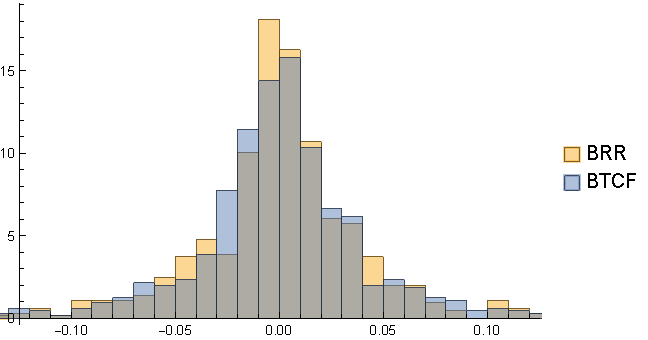
\includegraphics[scale=.7]{_pics/fittedNIG.pdf} 
  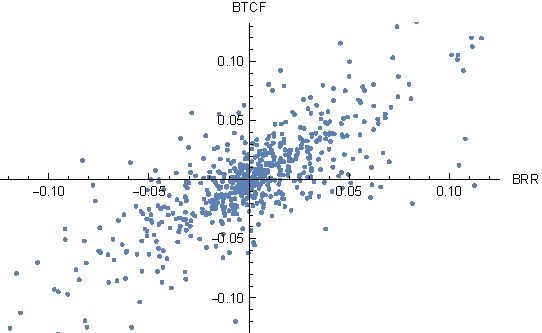
\includegraphics[scale=.7]{_pics/scatter.pdf}
  \caption{BRR and BTCF return distributions (empirical and fitted to
    NIG) as well as scatter plot.}
  \label{fig:nig}
\end{figure}

\subsubsection{Fitting the NIG factor copula}
\label{sec:fitting-nig-factor}

If the margins are not NIG-distributed, then the NIG factor copula
model is calibrated as follows. Denote the NIG distribution function
by $F(\cdot; \alpha, \beta, \mu, \delta)$. Denote the margins by
$U_i\sim U(0,1)$, $i=1,2$. The factor model of Proposition
\ref{prop:NIG} is 
obtained by transforming the uniform margins to standardised NIG
distributions by setting  
$X_i:=F^{(-1)}(U_i; \alpha, \beta, \mu, \delta+\delta_i)$ with 
$\delta+\delta_i=\displaystyle \frac{(\alpha^2-\beta^2)^{3/2}}
{\alpha^2}$ and $\mu=\displaystyle -\frac{(\delta+\delta_i)\beta}
{\sqrt{\alpha^2-\beta^2}} = -\frac{(\alpha^2-\beta^2) \beta}
{\alpha^2}=\frac{\beta^3}{\alpha^2}-\beta$. Here, $\delta$ refers to
the scaling factor of the latent variable $Z$. In 
this case, $\E X_i=0$ and $\text{Var}(X_i)=1$.


Denote the $r$-th
empirical uncentered moment of $i$-th NIG-transformed margin by
\begin{equation}
  \label{eq:8}
  \hat\mu_{i,r}(\alpha, \beta, \mu,\delta) := \frac{1}{n}
  \sum_{j=1}^n 
  F^{(-1)}(u_{i,j}; \alpha,\beta,\mu, \delta)^r,
\end{equation}



Given the interpretation of the parameters -- $\alpha$ as the tail
heaviness, $\beta$ as the degree of asymmetry, and $\delta$
determining the correlation -- calibrating the bivariate factor model
is the achieved by minimising the RMSE of the third and
fourth moments and the correlation between the model and the data: 
\begin{multline*}
  \min _{\alpha, \beta, \delta, \delta_1, \delta_2}
  \left(\text{Corr}(F^{(-1)}(U_1; \alpha, \beta, \mu,\delta+\delta_1),
  F^{(-1)}(U_2; \alpha, \beta, \mu, \delta+\delta_2)-\frac{\delta}
  {\sqrt{(\delta+\delta_1) (\delta+\delta_2)}}\right)^2\\
+ \sum_{i=1}^2 \sum_{r=3}^4 
  \left(\hat\mu_{i,r}(\alpha,\beta,\delta+\delta_i) -
    \frac{\partial^r}{\partial u^r} M(u; \alpha,  
    \beta,\mu, \delta+\delta_i)\Big|_{u=0}\right)^2 \text{, subject
    to } \delta+\delta_i=\displaystyle \frac{(\alpha^2-\beta^2)^{3/2}}
{\alpha^2},
\end{multline*}
with $\mu=\displaystyle\frac{\beta^3}{\alpha^2}-\beta$. 

This implies that $\delta_1=\delta_2$. A standardised multivariate
model would therefore be homogeneous with one correlation coefficient
for all pairwise margins. Different correlations would be achieved 
by loosening the constraint of unit variances. Re-writing, with
$\tilde\delta := \delta + \delta_1 = \displaystyle
\frac{(\alpha^2-\beta^2)^{3/2}} {\alpha^2}$ gives 
\begin{equation*}
  \min _{\alpha, \beta, \delta}
  \left(\text{Corr}(F^{(-1)}(U_1; \alpha, \beta, \mu,\tilde\delta),
  F^{(-1)}(U_2; \alpha, \beta, \mu, \tilde\delta)-\frac{\delta}
  {\tilde\delta}\right)^2 %
+ \sum_{i=1}^2 \sum_{r=3}^4 
  \left(\hat\mu_{i,r}(\alpha,\beta,\tilde\delta) -
    \frac{\partial^r}{\partial u^r} M(u; \alpha,  
    \beta,\mu, \tilde\delta) \Big|_{u=0}\right)^2.
\end{equation*}

\subsubsection{NIG quantiles}
\label{sec:nig-quantiles}

Calibrating the model requires an efficient implementation of the NIG
quantile function, see Equation (\ref{eq:8}. One way of implementing
this is via the so-called {\em Cornish-Fisher expansion}.

\natp{CF expansion here.}

\natp{Simulation produces better results but requires more
  computational power. Hence, use CF for calibration, which performs
  worse in the tails, and simulation in the hedge calculation / risk
  measure calculation. Use importance sampling.}


\subsubsection{Hedge calculation in the NIG factor model}
\label{sec:hedge-calc-nig}

Optimising for the hedge quantity $h$ requires fast calculations of
the hedge distribution function \eqref{eq:3}. The position obtained
from hedging Bitcoin with $h$ units of the Bitcoin future returns
\begin{equation*}
  R^h = X_1 - h X_2 = Z + Z_1 - h Z - h Z_2 = (1-h) Z + Z_1 - h Z_2,
\end{equation*}
with $Z, Z_1, Z_2$ independent NIG-distributed random
variables. Without loss of generally, set $\mu=0$. Because of the
scaling with $1-h$ and $h$, $R^h$ will not follow an NIG distribution,
unless $h=0$.  A direct calculation of the distribution function is
achieved by numerically computing the integral
\begin{equation*}
  \p(R^h\leq x) = \int_0^\infty \int_0^\infty \int_0^\infty
  \Ncdf(y; \mu_1 - h \mu_2 + \beta w_1 - h w_2, (1-h)^2 w + w_1 + h^2
  w_2)\, f_W(w)\, f_{W_1}(w_1)\, f_{W_2} (w_2)\, \dd w\, \dd w_1\, \dd w_2,
\end{equation*}
where $\Ncdf(x; \mu, \sigma^2)$ denotes the normal distribution
function with expectation $\mu$ and variance $\sigma^2$, and
$f_W, f_{W_1}, f_{W_2}$ are the inverse gamma density functions of the
scaling variables $W$, $W_1$ and $W_2$ with parameters
$\delta, \delta_1, \delta_2$ and $\sqrt{\alpha^2-\beta^2}$. 

However, for determining the optimal hedge parameter $h$, numerical
computation of the three-fold integral may be slow, compared to other
methods that make explicit use of the simple form of the
moment-generating function.  The following two methods achieve a much
faster computation for the NIG factor model.  The first method uses
Fourier inversion to calculate the density from the characteristic
function. The second method approximates the distribution of $R^h$ by
an NIG distribution.  Both methods use the moment-generating function
of $R^h$, which is given by
\begin{align}
  \varphi_h(u):=\E\left[\e^{u R^h}\right]
  &= \E\left[ \e^{u[(1-h) Z + Z_1 -h Z_2]}\right] %
    = \E\left[ \e^{u(1-h) Z}\right]\, \E\left[ \e^{u Z_1}\right] \,
    \E\left[ \e^{-u h Z_2}\right]\nonumber\\
  &=M\left(u;\frac{\alpha}{1-h}, \frac{\beta}{1-h}, (1-h)\mu,
    (1-h)\delta\right)\,
    M\left(u; \alpha, \beta, \mu_1, \delta_1\right)\,
    M\left(-u; \frac{\alpha}{h}, \frac{\beta}{h}, h\mu_2,
    h\delta_2\right).
    \label{eq:7}
\end{align}


\natp{Add copula stuff; here the assumption is still that $R_S$ and
  $R_F$ are NIG.}

\paragraph*{Calculation via Fourier inversion}
\label{sec:calc-via-four}

Because of the simple form of the moment-generating function
\eqref{eq:7}, the density $f$ of $R^h$ can be calculated numerically
using the inverse Fourier transform of the characteristic function
$\varphi(u) $:
\begin{equation*}
  f(x) = \frac{1}{2\pi} \int_\R \e^{-i u x} \varphi_h(u)\, \dd u, 
\end{equation*}
and the distribution function of $R^h$ can be calculated as
\begin{equation*}
  \p(R^h\leq x) = \lim_{b\rightarrow-\infty} \frac{1}{2\pi} \int_\R
  \frac{\e^{-i u x} - \e^{-i u b}}{i u}\, \varphi_h(u)\, \dd u,
\end{equation*}
see e.g.\ II.\S 12, Theorem 3 of \citep{Shiryaev1996}.


\paragraph*{NIG approximation of hedged position}
\label{sec:nig-appr-hedg}

If $h=1$ and $\beta=0$, then $R^h$ is NIG, hence, if $h$ is close to
$1$, it may be feasible to approximate $R^h$ by an NIG. The parameters
can be determined either by moment-matching or by a first-order Taylor
approximation of the moment-generating function's exponent.


For the moment-matching procedure, set
$R^h\approx \text{NIG}(\alpha_h, \beta_h, \mu_h, \delta_h)$ and solve
for $\alpha_h, \beta_h, \mu_h, \delta_h$, 
\begin{equation*}
  \begin{pmatrix}
    \frac{\partial}{\partial u} \varphi_h(u)\big|_{u=0}\\[5pt]
    \frac{\partial^2}{\partial u^2} \varphi_h(u)\big|_{u=0}\\[5pt]
    \frac{\partial^3}{\partial u^3} \varphi_h(u)\big|_{u=0}\\[5pt]
    \frac{\partial^4}{\partial u^4} \varphi_h(u)\big|_{u=0}
  \end{pmatrix}
  =
  \begin{pmatrix}
    \frac{\partial}{\partial u} M(u;\alpha_h, \beta_h, \mu_h,
    \delta_h)_{u=0}\\[5pt]
    \frac{\partial^1}{\partial u^2} M(u;\alpha_h, \beta_h, \mu_h,
    \delta_h)_{u=0}\\[5pt]
    \frac{\partial^2}{\partial u^3} M(u;\alpha_h, \beta_h, \mu_h,
    \delta_h)_{u=0}\\[5pt]
    \frac{\partial^3}{\partial u^4} M(u;\alpha_h, \beta_h, \mu_h,
    \delta_h)_{u=0}
  \end{pmatrix}.
\end{equation*}
% \begin{equation*}
%   \min_{\alpha_h, \beta_h, \mu_h, \delta_h} \sqrt{\sum_{r=1}^4
%     \left(\frac{\partial^r}{\partial u^r} \left[\E\left[\e^{u
%             R^h}\right] - M(u;\alpha_h, \beta_h, \mu_h,
%         \delta_h)\right]_{u=0}\right)^2}, 
% \end{equation*}
% allows for an efficient computation of

An alternative to determine the parameters is to assume that $h=1$ so
that $R^1 = Z_1 - Z_2$ and using the following first-order Taylor
approximation around zero: 
\begin{equation*}
  \sqrt{\alpha^2 -
    (\beta + u)^2}-\sqrt{\alpha^2 - (\beta - u)^2} \approx
  -\frac{2\beta}{\sqrt{\alpha^2 - \beta^2}}\, u. 
\end{equation*}
This gives 
\begin{align*}
  \varphi_1(u)
  &= M(u; \alpha, \beta, \mu_1, \delta_1) M(-u; \alpha, \beta, \mu_2,
    \delta_2) \\
  &= \exp\left(\delta_1 (\sqrt{\alpha^2-\beta^2} - \sqrt{\alpha^2 -
    (\beta+u)^2}) + \mu_1 \, u + \delta_2 (\sqrt{\alpha^2 - \beta^2} -
    \sqrt{\alpha^2 - (\beta - u)^2}) - \mu_2\, u\right)\\
  &= \exp\left(\delta_1 (\sqrt{\alpha^2-\beta^2} - \sqrt{\alpha^2 -
    (\beta+u)^2}) + \mu_1 \, u + \delta_2 (\sqrt{\alpha^2 - \beta^2} -
    \sqrt{\alpha^2 - (\beta + u)^2})  - \mu_2\, u\right)\\
  &\, \cdot \exp\left(\delta_2( \sqrt{\alpha^2 -
    (\beta + u)^2}-\sqrt{\alpha^2 - (\beta - u)^2})\right)\\
  &\approx \exp\left((\delta_1+\delta_2) (\sqrt{\alpha^2-\beta^2} -
    \sqrt{\alpha^2-(\beta+u)^2}) + \left(\mu_1-\mu_2
    -\frac{2\delta_2\beta}{\sqrt{\alpha^2-\beta^2}}\right) u\right)\\ 
  &= M\left(u; \alpha, \beta, \mu_1-\mu_2
    -\frac{2\delta_2\beta}{\sqrt{\alpha^2-\beta^2}},
    \delta_1+\delta_2\right). 
\end{align*}


\begin{figure}[t]
  \centering
  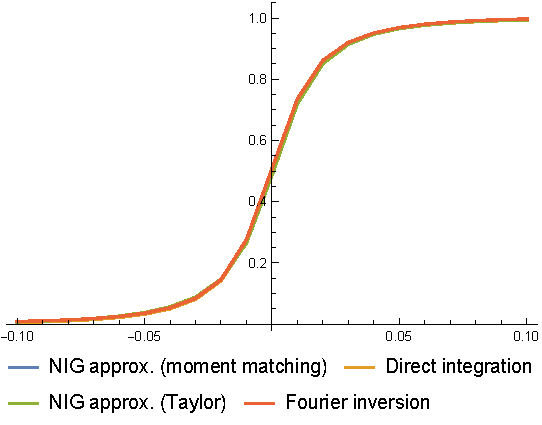
\includegraphics[scale=.8]{_pics/NIG1.pdf}
  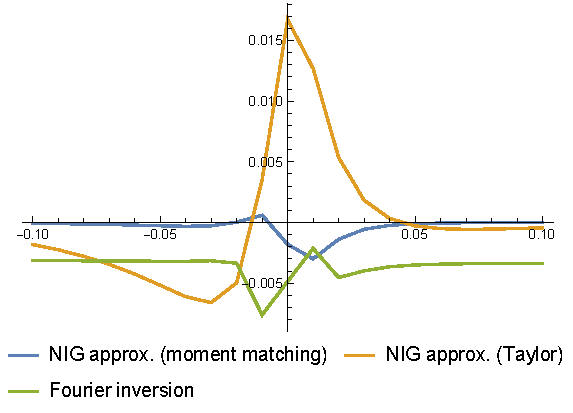
\includegraphics[scale=.8]{_pics/NIG2.pdf}
  \caption{Left: CDF of $R^{0.95}$ using Bitcoin data. Right:
    Difference of different methods to direct integration. CPU times:
    NIG approximation (moment matching): 0.2 seconds plus 18.6 seconds
    for parameter calibration; Direct integration: 82 seconds; NIG 
    approximation (Taylor): 0.18 seconds; Fourier inversion: 0.034
    seconds plus 1.55 seconds to generate smooth density function.}
  \label{fig:NIGs}
\end{figure}

Figure \ref{fig:NIGs} shows an example of the distribution of
$R^{0.95}$ for the different approximations as well as their error
relative to direct integration. It turns out that the NIG
moment-matching approximation performs best in terms of the error,
while the Taylor approximation performs worst. Taking into account CPU
times, the Fourier inversion technique performs best in terms of
balancing error and CPU time. 



\clearpage%
\natp{\em [The definition below is one way of introducing the
  elliptical copula, but not the most practical one for our
  purposes.]}

\begin{definition}
  Elliptical Distribution.  The $d$-dimensional random vector
  $\pmb{y}$ has an elliptical distribution if and only if the
  characteristic function
  $\pmb{t} \mapsto \mathbb{E}\{\exp(i\pmb{t}^\top \pmb{y})\}$ with
  $\pmb{t} \in \mathbb{R}^d$ has the representation
  \begin{align}
    \phi_g(\pmb{t}; \pmb{\mu}, \pmb{\Sigma}, \pmb{\nu}) = \exp(i\pmb{t}^\top\pmb{\mu})g(\pmb{t}^\top\pmb{\Sigma}\pmb{t};\pmb{\nu})
  \end{align}
  where $g(\cdot;\nu):[0, \infty[ \mapsto \mathbb{R}$,
  $\nu \in \mathbb{R}^d$, and $\Sigma$ is a symmetric positive
  semidefinite $d\times d$-matrix.
\end{definition}

If $r$ has a density, then the density of $\pmb{y}$ is of the form
\begin{align}
  |\Sigma|^{\frac{1}{2}} g\{(\pmb{y} - \pmb{\mu})^\top \Sigma^{-1}(\pmb{y} - \pmb{\mu})\}.
\end{align}

The function $g(\cdot; \nu)$ is known as characteristic generator,
whereas $\pmb{\nu}$ is parameter that determines the shape, in
particular the tai index of the distribution.





\begin{corollary} \citep[equation 2.12]{fang2018symmetric} If
  $\pmb{y}$ follows an elliptical distribution, then $\pmb{y}$ has a
  stochastic representation
  \begin{align}\label{eq:stochastic-representation}
    \pmb{y} = \pmb{\mu} + r\pmb{A}^\top \pmb{u},
  \end{align}
  where $r \in \mathbb{R}_+$ is independent of $\pmb{u}$
  % \footnote{$\pmb{u}$ is uniformly distributed on
  % $S_d = \{\pmb{u} \in \mathbb{R}^d s.t. ||\pmb{u}|| = 1\}$},
  , and $\pmb{A}^\top\pmb{A}=\pmb{\Sigma}$.
\end{corollary}

\begin{table}[ht]
  \center
  \begin{tabular}{lll}
    Distribution & $r \sim$ & $g(\pmb{t})$\\ \hline
    Gaussian & $\chi_n$ &
  \end{tabular}
  \caption{Generators of Elliptical Distributions summarised
    from~\cite[Chapter 2]{fang2018symmetric}}
  \label{tab:table}
\end{table}


\subsection{t-copulae}\label{subsec:t-copulae}
The t copula is to represent the dependency structure by t distribution~\citep{fang2002meta, embrechts2002correlation}.
\cite{demarta2005t} extend this idea to skewed t copula and grouped t copula to allow more flexibility in the modelling of dependency structure.

\subsubsection{Vanilla t-copula}\label{subsec:vanilla-t-copula}
The t-copula is
\begin{align}
    C^t_{\nu, \Sigma}(x) =
    \int_{-\infty}^{t_\nu^{-1}(x_1)} \dots \int_{-\infty}^{t_\nu^{-1}(x_n)}
    \frac{\Gamma\left\{ \frac{\nu + i}{2}\right\}}{\Gamma \left\{\frac{\nu}{2}\right\} (\pi \nu)^{i/2}|\Sigma|^{1/2}}
    \left(
    1+ \frac{y^\top \Sigma^{-1}y}{\nu}
    \right)^{-\frac{\nu + i}{2}}
    dy_1 \dots dy_n,
    \end{align}
where $t^{-1}_\nu$ is the quantile function of a univariate student-t distribution with degree of freedom $\nu$.

\subsubsection{Skewed t copula}\label{subsec:skewed-t-copula}
Mean variance mixture

\subsubsection{Double-t copula}\label{subsec:double-t-copula}
\natp{\em [It is OK to introduce the copula without any reference to CDO's.]}
\cite{hull2006valuing} present an alternative way to the Gaussian copula for valuing CDO tranches.
The double-t copula model is a weighted sum of a common (or market)
variable $M$ and a idiosyncratic variable $Z_i$. \natp{\em [They are
  $t$-distributed, right?]}
The double-t copula is
\begin{align} \label{eq:one-fator-model}
X_i = w_i M + \sqrt{1-w_i^2} Z_i
\end{align}
where $M$ and $Z_i$ are independent random variables with zero mean and unit variance, and $X_i$ is an indicator variable for $i^\text{th}$ asset.
The authors map the time to default of the $i^\text{th}$ obligor, $t_i$, to $X_i$,
\begin{align}
    F_{X_i}(x) = F_{t_i}(t).
    \end{align}
In our case, we map $X_i$ to log-returns of portfolio constituents,
\begin{align}
    F_{X_1}(x) = F_{r^S}(s) \text{ and } F_{X_2}(x) = F_{r^F}(t).
    \end{align}
This is also known as percentile-to-percentile
mapping\citep{hull2006defining}.

\natp{\em [The percentile-to-percentile mapping is just the property
  that applying the cdf to a random variable yields a $U(0,1)$
  variable:
  \begin{equation*}
    F(x) = \p(X\leq x) = \p(F(X) \leq F(x)) = \p(U\leq F(x)),
  \end{equation*}
  since by definition, $U\sim U(0,1)$ fulfills $\p(U\leq u)=u$, $0\leq
  u\leq 1$. This could be introduced when copulas and Sklar's Theorem
  are introduced. 
]}
The reason for this mapping is to turn incomprehensible dependency structures into known structure.

\subsubsection{Normal Inverse Gaussian Copula}
Normal Inverse Gaussian (NIG) distribution is a flexible 4-parameter distribution that can produce fat tails and skewness, unlike student-t distribution,
NIG's convolution is stable under certain conditions and the CDF, PDF and quantile function can still be computed sufficiently fast~\cite[chapter 5]{schlosser2011pricing}.
NIG distribution is a mixture of normal and inverse Gaussian distribution.
\begin{definition} Inverse Gaussian Distribution.
    A non-negative random variable $Y$ has an Inverse Gaussian (IG) distribution with parameters $\alpha >0$ and $\beta >0$ if its density funcion is of the form
    \begin{align}
        f_\text{IG}(y; \alpha, \beta) = \frac{\alpha}{\sqrt{2\pi \beta}}y^{-1.5} \exp\left\{
        -\frac{(\alpha - \beta z)^2}{2\beta z}
        \right\}
    \end{align}
    The corresponding distribution function is:
        \begin{align}
        F_\text{IG}(y; \alpha, \beta) = \frac{\alpha}{\sqrt{2\pi \beta}}
        \int_0^y z^{-1.5} \exp\left\{
        -\frac{(\alpha - \beta z)^2}{2\beta z}
        \right\}
            dz.
    \end{align}
    We write $Y \sim \text{IG}(\alpha, \beta)$.
    \end{definition}

\begin{definition} Normal Inverse Gaussian Distribution.
    A random variable $X$ has an Normal Inverse Gaussian (NIG) distribution with parameters $\alpha$, $\beta$, $\mu$ and $\delta$ if its density funcion is of the form
    \begin{align}
        X|Y=y &\sim \Phi(\mu + \beta y, y)\\
            Y &\sim \text{IG}(\delta \gamma, \gamma^2) \text{ with } \gamma \overset{\text{def}}{=}\sqrt{\alpha^2-\beta^2}
    \end{align}
    The corresponding distribution function is:
        \begin{align}
        F_\text{NIG}(y; \alpha, \beta) = \frac{\alpha}{\sqrt{2\pi \beta}}
        \int_0^y z^{-1.5} \exp\left\{
        -\frac{(\alpha - \beta z)^2}{2\beta z}
        \right\}
            dz.
    \end{align}
    \end{definition}


%%% Local Variables: 
%%% mode: latex
%%% TeX-master: "notes.tex"
%%% End: 




%\subsection{Extreme-value copulae}\label{subsec:extreme-value-copulae}
